\chapter{Teoría de Boltzmann}


El objetivo de la teoría cinética es describir las propiedades macroscópicas de los gases, tales como: presión, temperatura, conductividad térmica, viscosidad, etc; a partir de variables microscópicas que componen los gases como la velocidad, energía cinética e interacción entre otras. Los fundamentos de la teoría moderna fueron establecidos por Maxwell, quien propuso modelos estadísticos y un concepto de ecuación de transporte para poder modelar el comportamiento macroscópico. Esta teoría obtuvo un nuevo impulso a finales del siglo XIX con el trabajo de Boltzmann, quien propuso una ecuación integro-diferencial (ecuación de Boltzmann) la cual representa la evolución de la función de distribución en el espacio de fase. 

\medskip

\noindent Se consideran, en este trabajo, gases compuestos por una gran cantidad de moléculas las cuales se mueven independientemente unas de otras y colisionan entre sí o con las paredes del contenedor. Se asume también que las energías de interacción entre partículas son despreciables en comparación con sus energías cinéticas.

\section{Espacio de fase}

Para definir el espacio de fase se consideran N partículas en tres dimensiones con coordenadas generalizadas $q_{1}, ..., q_{3N}$ y momentos canónicamente conjugados  $p_{1}, ... , p_{3N}$. Llamamos espacio de fase $\Gamma$, al espacio que abarca $6N$ coordenadas. En este espacio, el estado del sistema a un tiempo dado $t$, es representado por un punto a partir de $6N$ valores, $3N$ debido a las componentes del vector de posición y $3N$ de las velocidades de las $N$ partículas.

\medskip

\noindent Generalmente los sistemas físicos que se estudian en la naturaleza se componen de una gran cantidad de partículas, de esta manera el espacio de fase tiene muchas dimensiones y es muy difícil determinar un punto en $\Gamma$. Para simplificar el estudio de la física a nivel macroscópico es necesario calcular cantidades como la energía, el volumen, etc. Estas se calculan conociendo un gran numero de micro estados, es decir, una colección de muchos puntos en el espacio de fase, sin embargo no será posible encontrar todos los micro estados y se hace necesario caracterizarlos mediante una función de distribución, adoptando una visión probabilística en $\Gamma$. 

\medskip

\noindent Un punto en el espacio de fase se escribe como $(q,p) = (q_{1}, ... ,q_{3N}, p_{1}, ... ,p_{3N})$ y se considera una densidad de probabilidad de ocurrencia en el tiempo t como $f(q,p,t)$. Esta distribución de probabilidad describe propiedades estadísticas de los estados en $\Gamma$ y permite analizar casos microscópicos dentro de resultados macroscópicos. En adelante el desafío será encontrar la función de distribución correspondiente a la situación física  particular. (\textbf{label seccion)}.

\medskip

\noindent Para un gran número de partículas N tenemos \cite{Schwabl}

\begin{eqnarray}
f(q,p,t)dqdp = f(q_{1}, ... , q_{3N},p_{1},..,p_{3N},t)\prod_{i=1}^{3N}dq_{i}dp_{i},
\end{eqnarray}

\noindent que representa la probabilidad de encontrar un sistema en un tiempo $t$, con un volumen en el espacio de fase $dqdp$, en la vecindad del punto $(q,p)$ en el espacio $\Gamma$. $f(q,p,t)$ es llamada la \textbf{función de distribución}, la cual debe ser positiva $f(q,p,t) \geq 0$ y normalizable. 

\begin{eqnarray}
f = f(\vec{r},\vec{v},t) \qquad f:{\rm I\!R}^{3}\times{\rm I\!R}^{3}\times{\rm I\!R}^{+}\longrightarrow{\rm I\!R}^{+}
\end{eqnarray}

%\section{Teorema de Louville}
%Se quiere determinar la dependencia temporal de la función de distribución 
%f(q,p,t), supongamos una distribución inicial $f(q_{o},p_{o})$ en $t = 0$


\section{Función de distribución de Maxwell}

La principal pregunta es, ¿cómo conocer la probabilidad de encontrar una molécula que se mueve en un rango de velocidades $\vec{v}+d\vec{v}$? Para poder responder tal pregunta se consideran tres suposiciones físicas \cite{lecture2}

\begin{itemize}
    \item[$\mathbf{\bullet}$] El número de partículas con velocidad $\vec{v}$ es proporcional a $d\vec{v}$. Entonces se considera que $\phi(\vec{v})d\vec{v}$ representa la probabilidad de encontrar una molécula con velocidad $\vec{v}$ en un rango $\vec{v} + d\vec{v}$
    
    \item[$\mathbf{\bullet}$] La probabilidad de encontrar partículas con velocidad $\vec{v}$ es independiente de los grados de libertad (en cada coordenada)

    \begin{eqnarray}
    \phi(u)du\ \phi(v)dv\ \phi(w)dw,
    \end{eqnarray}
    
    entonces se define una función de distribución que depende de las probabilidades de la siguiente manera
    
    \begin{eqnarray}
    f(u,v,w)dudvdw = n\phi(u)du\phi(v)dv\phi(w)dw,
    \end{eqnarray}
    
    donde $n$ denota la densidad de partículas dentro del diferencial del espacio de fase.
    
    \item[$\mathbf{\bullet}$] \textbf{Hipótesis de isotropía:} En el proceso de equilibrio, en ausencia de fuerzas externas, no se distingue entre las tres direcciones, es decir, se asume que las funciones de distribución tridimensionales se componen del producto de tres funciones unidimensionales
    
    \begin{eqnarray*}
    f(u,v,w) = n\phi(u)\phi(v)\phi(w) =\Phi(|\vec{v}|),
    \end{eqnarray*}
    
    entonces se toma el logaritmo para obtener
    
    \begin{eqnarray*}
    \ln \Phi(|\vec{v}|) = \ln n + \ln\phi(u)+\ln\phi(v)+\ln\phi(w),
    \end{eqnarray*}
    
    derivando para cada componente se obtiene un resultado interesante, que impone una condición de vital importancia
    
    
    \begin{eqnarray}
    \frac{1}{|\vec{v}|}\frac{d\ln\Phi(|\vec{v}|)}{d|\vec{v}|} = \frac{1}{u}\frac{d(\ln\phi(u))}{du}=\frac{1}{v}\frac{d\ln\phi(v)}{dv}=\frac{1}{w}\frac{d\ln\phi(w)}{dw},
    \end{eqnarray}
    
    la única posibilidad para que se cumplan las anteriores relaciones es que cada una sea igual a una constante. Integrando se llega a la siguiente expresión 
    
    \begin{eqnarray}
    \label{Fdistribucion}
    \phi(|\vec{v}|) = \alpha^{3} e^{-\beta v^{2}} \qquad\qquad  f(u,v,w) = n\alpha^{3}e^{-\beta v^{2}}
    \end{eqnarray}
    
    donde $\alpha$ y $\beta$ son constantes de integración postivas. Se elige negativo el exponente para que la función sea normalizable, es decir, sea una función de decreciemiento rápido, ideal para la descripción de cantidades físicas \cite{strichartz}.
    
    Ahora se determinan las constantes de integración en el equilibrio termodinámico, y así las variables de estado que se  utilizan son la densidad $\rho$ y la densidad de energía interna $\rho\epsilon$. 
    
    \begin{eqnarray}
    \label{rho}
    \rho(\vec{r},t) &=& mn = \int_{{\rm I\!R^{3}}}mf(\vec{r},\vec{v},t)d\vec{v}\\
    \label{denener}
    \rho(\vec{r},t)\epsilon &=& \frac{3}{2}nKT=\int_{{\rm I\!R^{3}}}\frac{1}{2}mv^{2}f(\vec{r},\vec{v},t)d\vec{v}
    \end{eqnarray}
    
    la ecuación \eqref{denener} expresa que la energía cinética de traslación promedio  por partícula está dada por el teorema de la equipartición de la energía. Integrando las anteriores expresiones y utilizando \eqref{Fdistribucion} se llega a las siguientes relaciones \footnote{Para calcular las integrales de la teoría cinética se puede utilizar la función Gamma 
    \begin{eqnarray}
    \int_{0}^{\infty}x^{n}e^{-\alpha x^{2}}dx = \frac{1}{2}\Gamma\left(\frac{n+1}{2}\right)\left(\frac{1}{\alpha}\right)^{\frac{n+1}{2}}
    \end{eqnarray}
     }
     
     \begin{eqnarray}
     \label{calculoint}
     \rho = \rho\alpha^{3}\left(\frac{\pi}{\beta}\right)^{3/2} , \qquad \frac{3}{2}nkT =\frac{3}{4}mn\alpha^{3}\left(\frac{\pi}{\beta}\right)^{3/2} \frac{1}{\beta}
     \end{eqnarray}
     
     encontrando,  a partir de las relaciones \eqref{calculoint},
     
     \begin{eqnarray}
     \boxed{
     \alpha = \left(\frac{m}{2\pi kT}\right)^{1/2}, \qquad \beta=\frac{m}{2kT}
     }
     \end{eqnarray}
    
    
    por lo tanto la función de distribución está dado por la siguiente expresión 
    
    \begin{eqnarray}
    f(\vec{r},\vec{v},t) = \rho(\vec{r},t)\left(\frac{m}{2\pi kT}\right)^{3/2}e^{-mv^{2}/2kT}.
    \end{eqnarray}

\end{itemize}

\noindent Esta es la distribución de Maxwell-Boltzmann , que modela la evolución en el tiempo de cada partícula en una posición y velocidad en particular. Sí se conoce $f$, las cantidades macroscópicas observables pueden calcularse a partir de funciones microscópicas. En particular se tienen los momentos macroscópicos  \cite{lecture1}

\begin{eqnarray}
\rho(\vec{r},t)&=&mn(\vec{r},t)=m\int_{{\rm I\!R}^{3}}f(\vec{r},\vec{v},t)d\vec{v}\\
\vec{u}(\vec{r},t) &=& \frac{1}{n(\vec{v},t)}\int_{{\rm I\!R}^{3}}\vec{v} f(\vec{r},\vec{v},t)d\vec{v}
\end{eqnarray}

\noindent que son respectivamente la densidad de masa y la densidad de velocidad. Ahora definimos la energía traslacional de la forma

\begin{eqnarray}
\epsilon(\vec{r},t)=\frac{1}{n(\vec{r},t)}\int_{{\rm I\!R}^{3}}(\vec{v}-\vec{u})^{2}f(\vec{r},\vec{v},t)d\vec{v}
\end{eqnarray}




\section{Ecuación de Boltzmann}



\noindent La función de distribución $f$ depende  de $\vec{x}$, $\vec{\xi}$ y $t$. Veamos su variación temporal

\begin{eqnarray}
\frac{df}{dt} = \left(\frac{\partial f}{\partial x_{\alpha}}\right)\frac{dx_{\alpha}}{dt}+\left(\frac{\partial f}{\partial \xi_{\alpha}}\right)\frac{d\xi_{\alpha}}{dt}+\left(\frac{\partial f}{\partial t}\right)
\end{eqnarray}

\noindent En donde $dx_{\alpha}/dt$ es la velocidad de las partículas a nivel mesoscópico $\xi_{\alpha}$. Por otro lado, el segundo término está relacionado con la aceleración y así, teniendo en cuenta la segunda ley de Newton, podemos escribir la densidad de fuerza como $d\xi_{\alpha}/dt = F_{\alpha}/\rho$. Por lo tanto la ecuación de evolución que tenemos está dada por 

\begin{eqnarray}
\frac{df}{dt} = \xi_{\alpha}\left(\frac{\partial f}{\partial x_{\alpha}}\right)+\frac{F_{\alpha}}{\rho}\left(\frac{\partial f}{\partial \xi_{\alpha}}\right)+\frac{\partial f}{\partial t}
\end{eqnarray}

\noindent en general, el lado izquierdo de la ecuación es un término fuente que indica la tasa de cambio de la función de distribución dada por las colisiones entre partículas.  La siguiente ecuación es llamada \emph{Ecuación de Boltzmann}

\begin{eqnarray}
\label{Boltzmann}
\frac{\partial f}{\partial t} + \xi_{\alpha}\left(\frac{\partial f}{\partial x_{\alpha}}\right)+\frac{F_{\alpha}}{\rho}\left(\frac{\partial f}{\partial \xi_{\alpha}}\right)=\Omega(f)
\end{eqnarray}

\noindent donde se ha definido el operador de colisión al termino $\Omega(f)$ el cual puede tener diversas formas, existe un amplio campo de investigación al respecto \cite{lecture3}\cite{lecture4}\cite{lecture5}. Sin embargo debemos exigir a tal operador que conserve tres cantidades físicas importantes, la masa, el momento y la energía. Matemáticamente se expresan como sigue 

\begin{eqnarray}
\int\Omega(f)d\vec{\xi} = 0 \qquad \int\vec{\xi}\Omega(f)d\vec{\xi} = 0 \qquad \int\xi^{2}\Omega(f)d\vec{\xi} = 0.
\end{eqnarray}

\noindent para deducir el operador de colisión se necesita resolver dos  integrales complicadas sobre todo el espacio \cite{lecture5}, que en esencia es considerar todas las posibles formas de colisión que puedan tener las partículas en estudio para una fuerza en particular. Un operador que cumple con tales condiciones fue el propuesto por Bhatnagar, Gross y Krook en 1954 \cite{BGK}, entonces se asume que 

\begin{eqnarray}
\Omega(f) = -\frac{1}{\tau}(f-f^{(0)})
\end{eqnarray}

\noindent en la anterior ecuación $\tau$ es el tiempo de relajación, el cual cuantifica que tan rápido chocan las partículas 

\section{Ecuaciones de conservación macroscópicas}

\noindent Tomando los momentos de la ecuación de Boltzmann \eqref{Boltzmann} se pueden encontrar las ecuaciones de conservación del sistema tales como la masa, el momento y la energía. Se define entonces

\begin{eqnarray}
\label{momentos}
\Pi_{o} = \int f d\vec{\xi} = \rho &\qquad& \Pi_{\alpha} = \int \xi_{\alpha}f d\vec{\xi} = \rho u_{\alpha}\\
\Pi_{\alpha\beta} = \int \xi_{\alpha\beta}f d\vec{\xi}  &\qquad& \Pi_{\alpha\beta\gamma} = \int \xi_{\alpha}\xi_{\beta}\xi_{\gamma}f d\vec{\xi} \nonumber
\end{eqnarray}

\noindent Para la conservación de la masa se integra \eqref{Boltzmann} obteniendo. 

\begin{eqnarray}
\frac{\partial}{\partial t}\int f d\vec{\xi}+\frac{\partial}{\partial x_{\alpha}}\int \xi_{\alpha}fd\vec{\xi}+\frac{F_{\alpha}}{\rho}\int \frac{\partial f}{\partial \xi_{\alpha}}d\vec{\xi} = \int \Omega(f)d\vec{\xi}
\end{eqnarray}

\noindent Notando que $t$ y $x$ no son funciones de $\xi$, podemos permutar la integral con la divergencia y reorganizar términos. Falta hacer el calculo del término de fuerza utilizando la integración por partes multidimensional\footnote{Ecuacion de integración por partes multidimensional \begin{eqnarray}
\label{partes}
\int_{V} \frac{\partial u}{\partial x_{\alpha}} = \int_{S}uv dS_{\alpha} - \int_{V}u\frac{\partial v}{\partial x_{\alpha}}\nonumber
\end{eqnarray}
} y asumiendo que las integrales de superficie se desvanecen cuando $\vec{\xi}\rightarrow  0$. Se impone esta última condición para asegurar que las ecuaciones de conservación sean finitas. Entonces se llega a la siguiente ecuación utilizando \eqref{momentos}


\begin{eqnarray}
\boxed{\frac{\partial \rho}{\partial t} +\frac{\partial \rho u_{\alpha}}{\partial x_{\alpha}}= 0 }
\end{eqnarray}

\noindent que es la ecuación de continuidad \cite{Landau}. La importancia de este resultado radica en que la forma de la ecuación de continuidad se mantendrá sin importar la forma funcional especifica de la función distribución, de tal manera que la definición de los momentos en la ecuación tienen mayor relevancia debido a que conectan el mundo mesoscópico con las ecuaciones macroscópicas.

\medskip

\noindent Para el caso de la siguiente ecuación de conservación se toma el primer momento de \eqref{Boltzmann} y se hace la integral en todo el espacio de velocidades, obteniendo la siguiente relación 



\begin{eqnarray}
\frac{\partial}{\partial t}\int \xi_{\alpha}f d\vec{\xi}+\frac{\partial}{\partial x_{\beta}}\int \xi_{\alpha}\xi_{\beta}fd\vec{\xi}+\frac{F_{\beta}}{\rho}\int \xi_{\alpha}\frac{\partial f}{\partial \xi_{\beta}}d\vec{\xi} = \int \xi_{\alpha}\Omega(f)d\vec{\xi}
\end{eqnarray}

\noindent Se utiliza la integración por partes para encontrar el momento relacionado con el término de la fuerza, encontrando que se puede hacer 

\begin{eqnarray}
\int \xi_{\alpha}\frac{\partial f}{\partial \xi_{\beta}}d\vec{\xi} = -\int \frac{\partial \xi_{\alpha}}{\partial \xi_{\beta}}fd\vec{\xi}= -\rho\delta_{\alpha\beta}
\end{eqnarray}

\noindent como resultado podemos ver la ecuación de conservación del momento dada por la siguiente expresión 

\begin{eqnarray}
\frac{\partial (\rho u_{\alpha})}{\partial t}+\frac{\partial \Pi_{\alpha\beta}}{\partial x_{\beta}} = F_{\alpha}
\end{eqnarray}

\noindent dada la definición de $\Pi_{\alpha\beta}$ dada en \eqref{momentos} podemos entender físicamente como el flujo de cantidad de movimiento dirección $\alpha$ de la dirección $\beta$ de momento, en donde se evidencia que es simétrica respecto de índices. Veamos con más detalle $\Pi_{\alpha\beta}$ , definamos $\xi_{\alpha}\xi_{\beta}=(u_{\alpha}+v_{\alpha})(u_{\beta}+v_{\beta})$, entonces obtenemos lo siguiente 

\begin{eqnarray}
\Pi_{\alpha\beta} = \int (u_{\alpha}u_{\beta}+u_{\alpha}v_{\beta}+v_{\alpha}u_{\beta}+v_{\alpha}v_{\beta})fd\vec{\xi} = \rho u_{\alpha}u_{\beta} -\sigma_{\alpha}
\end{eqnarray}

\noindent tomando la condición de simetría de el primer momento $\Pi_{\alpha\beta}=\Pi_{\beta\alpha}$ se encuentra  que $u_{\alpha}v_{\beta} + v_{\alpha}u_{\beta}=0$, esto hace que los términos intermedios de la anterior integral se cancelen, obteniendo los dos términos de la do derecho bajo esta definición de $\sigma$

\begin{eqnarray}
\sigma_{\alpha\beta} = - \int v_{\alpha}v_{\beta}fd\vec{\xi}
\end{eqnarray}

\noindent el cual representa la difusión del momento y está determinado por la forma que se eliga de f, finalmente se tiene

\begin{eqnarray}
\boxed{\frac{\partial (\rho u_{\alpha})}{\partial t}+\frac{\partial(\rho u_{\alpha}u_{\beta})}{\partial x_{\beta}}=\frac{\partial \sigma_{\alpha\beta}}{\partial x_{\beta}}+F_{\alpha}}
\end{eqnarray}

\noindent como última consideración encontramos la ecuación de conservación de energía , tomando el segundo momento de la función de distribución de la ecuación de Boltzmann \eqref{Boltzmann}

\begin{eqnarray}
\frac{\partial}{\partial t}\int \xi_{\alpha}\xi_{\beta}f d\vec{\xi}+\frac{\partial}{\partial x_{\alpha}}\int \xi_{\alpha}\xi_{\beta}\xi_{\gamma}fd\vec{\xi}+\frac{F_{\alpha}}{\rho}\int \xi_{\alpha}\xi_{\beta}\frac{\partial f}{\partial \xi_{\alpha}}d\vec{\xi} = \int \xi_{\alpha}\xi_{\beta}\Omega(f)d\vec{\xi}
\end{eqnarray}

\noindent que por las definiciones de momentos \eqref{momentos} encontramos una ecuación de conservación del siguiente estilo 


\begin{eqnarray}
\frac{\partial (\rho E)}{\partial t} + \frac{1}{2}\frac{\partial \Pi_{\alpha\beta\gamma}}{\partial x_{\alpha}}=F_{\alpha}u_{\alpha}
\end{eqnarray}

En donde $\Pi_{\alpha\beta\gamma}$ representa el flujo de energía en la dirección $\alpha$. Tomando en cuenta el desarrollo en la deducción de el primer momento, calculamos 

\begin{eqnarray}
\frac{1}{2}\Pi_{\alpha\beta\gamma}&=&\frac{1}{2}\int (u_{\alpha}u_{\beta}u_{\gamma}+u_{\alpha}u_{\beta}u_{\gamma}+u_{\alpha}u_{\beta}u_{\gamma}+u_{\alpha}u_{\beta}u_{\gamma})fd\vec{\xi}\nonumber\\
&=&\frac{1}{2}\rho u_{\alpha} u^{2}+\rho u_{\alpha}e- u_{\beta}\sigma_{\alpha\beta}+q_{\alpha}\nonumber\\
&=&\rho u_{\alpha}E - u_{\beta}\sigma_{\alpha\beta} +q_{\alpha}
\end{eqnarray}

\noindent se tiene ahora que el primer término representa la advección macroscópica de la energía, el segundo término como el trabajo hecho por el tensor de "Strain" y se define el último termino como la difusión de la energía de la siguiente manera

\begin{eqnarray}
q_{\alpha} = \frac{1}{2}\int v_{\alpha} v^{2}f d\vec{\xi}
\end{eqnarray}

Finalmente se llega a la ecuación de conservación relacionada con la energía

\begin{eqnarray}
\boxed{
\frac{\partial (\rho e)}{\partial t} + \frac{\partial (\rho u_{\alpha}e)}{\partial x_{\alpha}}= \sigma_{\alpha\beta}\frac{\partial (\sigma_{\alpha\beta}u_{\beta})}{\partial x_{\alpha}}+ F_{\alpha}u_{\alpha}-\frac{\partial q_{\alpha}}{\partial x_{\alpha}}
}
\end{eqnarray}



\section{Expansión de Chapman-Enskog}

\noindent La dinámica macroscópica del fluido se puede ver como el resultado de un comportamiento colectivo de las partículas microscópicas en el sistema de estudio. Naturalmente el formalismo que describe esto de manera adecuada serán las ecuaciones de Navier Stokes\eqref{NS} con las consideraciones de conservación, para poder llegar a las ecuaciones macroscópicas a partir del método de Lattice Boltzmann se utiliza una perturbación del equilibrio. Para empezar a introducir este formalismo de manera más clara, se debe considerar la ecuación de Boltzmann\eqref{Boltzmann} sin dimensión  esto con el fin de entender de mejor manera las escalas en las cuales se posiciona nuestro sistema. Vamos a denotar las cantidades sin dimensión con $\widetilde{x}$ y un número característico apropiado , definimos

\begin{eqnarray}
\widetilde{t} &=& \frac{\xi_{o}}{x_{o}} t \qquad \widetilde{x} = \frac{x}{x_{o}}\qquad \widetilde{\xi}=\frac{\xi}{\xi_{o}}\nonumber\\
\widetilde{\tau} &=& \frac{\xi_{o}}{\overline{x}}\tau\qquad \widetilde{F} = \frac{x_{o}}{\rho\xi_{o}^{2}}F\qquad \widetilde{f} = \frac{c_{o}^{3}}{\rho}f
\end{eqnarray}

\noindent cuando se utilizan las anteriores definiciones sobre la ecuación de Boltzmann se encuentra que en terminos de las variables sin dimensiones se llega a la siguiente ecuación de Boltzmann sin dimensiones

\begin{eqnarray}
\frac{\overline{x}}{x_{o}}\left(\frac{\partial \widetilde{f}}{\partial \widetilde{t}}+\widetilde{\xi}_{\alpha}\frac{\partial \widetilde{f}}{\partial \widetilde{x}_{\alpha}}+\widetilde{F}_{\alpha}\frac{\partial \widetilde{f}}{\partial \widetilde{\xi}_{\alpha}}\right)=-\frac{1}{\widetilde{\tau}}\left(\widetilde{f}-\widetilde{f}^{(0)}\right)
\end{eqnarray}

\noindent entonces se encuentra el numero de Knudsen 

\begin{eqnarray}
\label{Kn}
\text{Kn} = \frac{\overline{x}}{x_{o}}=\frac{\overline{t}}{t_{o}}
\end{eqnarray}

\noindent en donde $\overline{x}$ es el camino libre medio y $\overline{t} = \overline{x}/\xi_{o}$ el tiempo libre medio. Sí $\text{Kn}\rightarrow0$ ambos lados de la ecuación van a cero, el lado izquierdo por la definición del numero de Knudsen, por otro lado, el lado izquierdo se anula porque la función de distribución es muy parecida a la función de equilibrio. Vemos que en cuanto Kn se hace más grande se desvía del equilibrio el sistema, entonces se introduce un pequeño parámetro $\epsilon$ para hacer una expansión y poder perturbar la ecuación de Boltzmann, entonces se introduce

\begin{eqnarray}
f_{i} = \sum_{n=0}^{+\infty}\epsilon^{n}f_{i}^{(n)}\qquad \frac{\partial}{\partial t} = \sum_{n=0}^{+\infty}\epsilon^{n}\frac{\partial}{\partial t_{n}}\qquad\frac{\partial}{\partial x_{\alpha}} = \sum_{n=0}^{+\infty}\epsilon^{n}\frac{\partial}{\partial x_{\alpha}^{n}}\qquad\frac{\partial}{\partial \xi_{\alpha}} = \sum_{n=0}^{+\infty}\epsilon^{n}\frac{\partial}{\partial \xi_{\alpha}^{n}}
\end{eqnarray}

\noindent el primer paso para poder discretizar la ecuación de Boltzmann es poder poner la velocidad en vectores discretos, para esto se utiliza una proyección en la base de hermite de la funcion de distribución de Boltzmann \cite{kruger}. Encontramos que la función de equilibrio discreta tiene la siguiente forma 

\begin{eqnarray}
\label{equilibrio}
\boxed{
f_{i}^{(0)} = \rho w_{i}\left(1+\frac{\xi_{i\alpha}u_{\alpha}}{c_{o}^{2}}+\frac{\xi_{i\alpha}\xi_{i\beta}u_{\alpha}u_{\beta}}{2c_{o}^{4}}-\frac{u_{\alpha}u_{\alpha}}{2c_{o}^{2}}\right)
}
\end{eqnarray}

\noindent en este caso consideramos la parte clásica de los fluidos, porque consideramos la ecuación discreta sin termino de forzamiento, entonces estamos trabajando sobre un formalismo para poder simular las ecuaciones de Navier Stokes 

\begin{eqnarray}
\label{latticeFluidos}
\boxed{\frac{\partial f_{i}}{\partial t}+\xi_{i\alpha}\frac{\partial f_{i}}{\partial x_{\alpha}}=-\frac{1}{\tau}\left(f_{i}-f_{i}^{(0)}\right)}
\end{eqnarray}

Ahora para poder tener la parte discreta de la anterior ecuación se usa el teorema fundamental del cálculo, obteniendo 

\begin{eqnarray}
f_{i}(\vec{x}+\vec{\xi}\Delta t, t + \Delta t)&-&f_{i}(\vec{x},t) \nonumber\\
&=&- \frac{1}{\tau}\int_{0}^{\Delta t}[f_{i}(\vec{x}+\vec{\xi}\lambda, t + \lambda)-f_{i}^{(0)}(\vec{x}+\vec{\xi}\lambda, t + \lambda)]d\lambda
\end{eqnarray}

\noindent para los cálculos utilizados en estos estudios se utiliza el primer orden de discretización entonces se utiliza la siguiente ecuación 


\begin{eqnarray}
\label{LBdiscreta}
f_{i}(\vec{x}+\vec{\xi}\Delta t, t + \Delta t)-f_{i}(\vec{x},t)  
=- \frac{1}{\tau}[f_{i}(\vec{x}, t)-f_{i}^{(0)}(\vec{x}, t)]
\end{eqnarray}


El resultado es explícito en el tiempo, el valor de la función de distribución en el siguiente paso depende del paso actual



\section{Fluidos}

Cuando se considera la ecuación discreta \eqref{latticeFluidos} se debe escoger un conjunto de velocidades discretas adecuadas para poder solucionar tal ecuación, a partir de la definición de los momentos \eqref{momentos} macroscópicos podemos plantear expresiones que permitan calcular las características del fluidos cuando estamos en el sistema discreto, por ejemplo 

\begin{eqnarray}
\label{densidad}
\sum_{i}f_{i}^{(0)}(\vec{x},t) &=& \rho(\vec{x},t)\\
\label{momento}
\sum_{i}\xi_{i\alpha}f_{i}^{(0)}(\vec{x},t) &=& \rho(\vec{x},t)u_{\alpha}(\vec{x},t)\\
\label{momento2}
\sum_{i}\xi_{i\alpha}\xi_{i\beta}f_{i}^{(0)}(\vec{x},t) &=& \Pi_{\alpha\beta}^{(0)}(\vec{x},t)\\
\label{momento3}
\sum_{i}\xi_{i\alpha}\xi_{i\beta}\xi_{i\gamma}f_{i}^{(0)}(\vec{x},t) &=& \Pi_{\alpha\beta\gamma}^{(0)}(\vec{x},t)
\end{eqnarray}

\noindent estas definiciones nos ayudan a imponer condiciones sobre la velocidad discreta, que hace que el sistema físico cobre sentido, vamos a utilizar las anteriores ecuaciones para deducir tales condiciones y la función de equilibrio propuesta \eqref{equilibrio}, lo primero será utilizar la densidad, en este caso 

\begin{eqnarray}
\rho &=& \sum_{i}f_{i}^{0}\nonumber\\
&=&\rho\left[\sum_{i}w_{i}+\frac{u_{\alpha}}{c_{o}^{2}}\sum_{i}w_{i}\xi_{i\alpha}+\frac{u_{\alpha}u_{\beta}}{2c_{o}^{4}}\sum_{i}w_{i}\xi_{i\alpha}\xi_{i\beta}-\frac{u_{\alpha}u_{\alpha}}{2c_{o}^{2}}\sum_{i}w_{i}\right]
\end{eqnarray}


\noindent para que las expresiones sean iguales el termino entre paréntesis cuadrados debe ser cero, entonces resultan las siguientes condiciones 

\begin{eqnarray}
\label{condicion1}
\sum_{i}w_{i}=1\qquad \sum_{i}w_{i}\xi_{i\alpha} = 0 \qquad \sum_{i}w_{i}\xi_{i\alpha}\xi_{i\beta}=c_{o}^{2}\delta_{\alpha\beta}
\end{eqnarray}

\noindent son las tres primeras condiciones para las velocidades y pesos utilizando el momento cero . Ahora se utiliza el primer momento, entonces se tiene

\begin{eqnarray}
\rho u_{\alpha} &=& \sum_{i}\xi_{i\alpha}f_{i}^{(0)}\nonumber\\
&=&\rho\left[\cancelto{0}{\sum_{i}w_{i}\xi_{i\alpha}}+\frac{u_{\alpha}}{c_{o}^{2}}\sum_{i}w_{i}\xi_{i\alpha}\xi_{i\beta}+\frac{u_{\alpha}u_{\beta}}{2c_{o}^{2}}\sum_{i}w_{i}\xi_{i\alpha}\xi_{i\beta}\xi_{i\gamma}-\frac{u_{\alpha}u_{\alpha}}{2c_{o}^{2}}\cancelto{0}{\sum_{i}w_{i}xi_{i\alpha}}\quad\right]\nonumber\\
&=&\rho\underbrace{\left[\frac{u_{\alpha}}{c_{o}^{2}}\sum_{i}w_{i}\xi_{i\alpha}\xi_{i\beta}+\frac{u_{\alpha}u_{\beta}}{2c_{o}^{2}}\sum_{i}w_{i}\xi_{i\alpha}\xi_{i\beta}\xi_{i\gamma}\right]}_{u_{\alpha}}
\end{eqnarray}

Utilizando la última ecuación de \eqref{condicion1} se hace necesario imponer la siguiente condición para poder obtener el momento macroscópico

\begin{eqnarray}
\label{condicion2}
\sum_{i}w_{i}\xi_{i\alpha}\xi_{i\beta}\xi_{i\gamma} = 0 
\end{eqnarray}

\noindent por último se utiliza la condición del segundo momento para evidenciar la última condición que consideramos 

\begin{eqnarray}
\Pi_{\alpha\beta}^{0}&=&\rho u_{\alpha}u_{\beta}+\rho c_{o}^{2}\delta_{\alpha\beta}=\sum_{i}\xi_{i\alpha}\xi_{i\beta}f_{i}^{(0)}\nonumber\\
&=&\rho\left[\sum_{i}w_{i}\xi_{i\alpha}\xi_{i\beta} + \frac{u_{\gamma}}{c_{o}^{2}}\cancelto{0}{\sum_{i}w_{i}\xi_{i\alpha}\xi_{i\beta}}\xi_{i\gamma}+\frac{u_{\gamma}u_{\phi}}{2c_{o}^{4}}\sum_{i}w_{i}\xi_{i\alpha}\xi_{i\beta}\xi_{i\gamma}\xi_{i\phi}-\frac{u_{\gamma}u_{\gamma}}{2c_{o}^{2}}\sum_{i}w_{i}\xi_{i\alpha}\xi_{i\beta}\right]\nonumber\\
&=&\rho c_{o}^{2}\delta_{\alpha\beta}\underbrace{+\frac{u_{\gamma}u_{\phi}}{2c_{o}^{4}}\sum_{i}w_{i}\xi_{i\alpha}\xi_{i\beta}\xi_{i\gamma}\xi_{i\phi}-\frac{u_{\gamma}u_{\gamma}}{2}\delta_{\alpha\beta}}_{=\rho u_{\alpha}u_{\beta}}
\end{eqnarray}

\noindent utilizando la ayuda de la delta de kronecker se puede exigir la condición del momento de la siguiente manera, completando las condiciones sobre las velocidades y los pesos

\begin{eqnarray}
\sum_{i}w_{i}\xi_{i\alpha}\xi_{i\beta}\xi_{i\gamma}\xi_{i\phi} = c_{o}^{4}(\delta_{\alpha\beta}\delta_{\gamma\phi}+\delta_{\alpha\gamma}\delta_{\beta\phi}+\delta_{\alpha\phi}\delta_{\beta\gamma})
\end{eqnarray}

\noindent hasta el momento se tienen las condiciones para poder encontrar el conjunto de velocidades que respete las definiciones macroscópicas. Ahora para poder tener la parte discreta de la ecuacion de Boltzmann \eqref{LBdiscreta} se hace una expansión en serie de Fourier de la ecuación de evolución del sistema 

\begin{eqnarray}
\label{expansion}
f_{i}(\vec{x}+\vec{\xi_{i}}\Delta t, t + \Delta t)-f_{i}(\vec{x},t) = \Delta t \frac{\partial f_{i}}{\partial x_{\alpha}}\xi_{i\alpha} &+& \Delta t \frac{\partial f_{i}}{\partial t} + \frac{\Delta t^{2}}{2}\frac{\partial^{2}f_{i}}{\partial x_{\alpha} \partial x_{\beta}}\xi_{i\alpha}\xi_{i\beta}+\nonumber\\\frac{\Delta t^{2}}{2}\frac{\partial^{2}f_{i}}{\partial t^{2}}
&+& \Delta t^{2} \frac{\partial^{2}f_{i}}{\partial x_{\alpha}\partial t}\xi_{i\alpha} = -\frac{1}{\tau}(f_{i}-f^{eq}_{i})
\end{eqnarray}

\noindent en donde los índices griegos denotan la dimensión del sistema en estudio. Para reproducir las ecuaciones de Navier-Stokes se aplica una expansión de Chapman-Enskog usando un parámetro $\epsilon$


\begin{eqnarray}
f_{i} = \sum_{n=0}^{\infty} \epsilon^{n} f_{i}^{(n)}, \qquad \frac{\partial}{\partial t} = \sum_{n = 0}^{\infty}\epsilon^{n}\frac{\partial}{\partial t_{n}}
\end{eqnarray}

\noindent Tomando el número de Knudsen\eqref{Kn} se puede identificar que el parámetro perturvativo $\epsilon = \Delta t$ en la ecuación de Boltzmann discretizada\eqref{LBdiscreta} \cite{principal} en donde, ahora reemplazando en la expansión de Taylor \eqref{expansion}  las definiciones de los términos perturvativos se tiene que 

\begin{eqnarray}
&\Delta t&\left(\xi_{i\alpha}\frac{\partial}{\partial x_{\alpha}}\left(f_{i}^{(0)}+\epsilon f_{i}^{(1)} + \epsilon^{2} f_{i}^{(2)}\right) + \left(\frac{\partial}{\partial t_{0}} + \epsilon \frac{\partial}{\partial t_{1}} \right)\left(f_{i}^{(0)}+\epsilon f_{i}^{(1)} + \epsilon^{2} f_{i}^{(2)}\right)\right)\nonumber \\
&+&\frac{\Delta t^{2}}{2}\left(\xi_{i\alpha}\xi_{i\beta}\frac{\partial^{2}}{\partial x_{\alpha}\partial x_{\beta}}\left(f_{i}^{(0)}+\epsilon f_{i}^{(1)} + \epsilon^{2} f_{i}^{(2)}\right)+\left(\frac{\partial}{\partial t_{0}} + \epsilon \frac{\partial}{\partial t_{1}} \right)^{2}\left(f_{i}^{(0)}+\epsilon f_{i}^{(1)} + \epsilon^{2} f_{i}^{(2)}\right)\right)\nonumber \\
&+&\frac{\Delta t^{2}}{2}\left(\xi_{i\alpha}\left(\frac{\partial}{\partial x_{\alpha}}\right)\left(\frac{\partial}{\partial t_{0}} + \epsilon \frac{\partial}{\partial t_{1}} \right)\left(f_{i}^{(0)}+\epsilon f_{i}^{(1)} + \epsilon^{2} f_{i}^{(2)}\right)\right) \nonumber\\
&=& -\frac{1}{\tau}\left(\left(f_{i}^{(0)}+\epsilon f_{i}^{(1)} + \epsilon^{2} f_{i}^{(2)}\right)-f_{i}^{eq}\right)
\end{eqnarray}

\noindent si se compara los términos de orden cero, uno y dos se pueden encontrar las siguientes relaciones 

\begin{eqnarray}
\label{momento0}
f_{i}^{0} &=& f_{i}^{eq} \\
\label{momento1}
\frac{\partial f_{i}^{(0)}}{\partial t_{0}} &+& \xi_{i\alpha}\frac{\partial f_{i}^{(0)}}{\partial x_{\alpha}} = -\frac{f_{i}^{(1)}}{\tau} \\
\xi_{i\alpha}\frac{\partial f_{i}^{(1)}}{\partial x_{\alpha}} + \frac{\partial f_{i}^{(1)}}{\partial t_{0}} &+& \frac{\xi_{i\alpha}\xi_{i\beta}}{2}\frac{\partial^{2}f_{i}^{(0)}}{\partial x_{\alpha}\partial x_{\beta}}+\frac{1}{2}\frac{\partial^{2}f_{i}^{(0)}}{\partial t_{0}^{2}}+\nonumber \\
\xi_{i\alpha}\frac{\partial^{2}f_{i}^{(0)}}{\partial t_{0}^{2}}&+&\xi_{i\alpha}\frac{\partial^{2}f_{i}^{(0)}}{\partial x_{\alpha}\partial t_{0}}+\frac{\partial f_{i}^{(0)}}{\partial t_{1}} = -\frac{f_{i}^{(2)}}{\tau} 
\end{eqnarray}

\noindent a partir de \eqref{momento0} y las siguientes sustituciones considerando \eqref{momento1}

\begin{eqnarray}
\xi_{i\alpha}\frac{\partial f_{i}^{(0)}}{\partial x_{\alpha}} = -\frac{f_{i}^{(1)}}{\tau}-\frac{\partial f_{i}^{(0)}}{\partial t_{0}}, \qquad \frac{\partial^{2} f_{i}^{(0)}}{\partial t_{0}^{2}}=-\frac{1}{\tau}\frac{\partial f_{i}^{(1)}}{\partial t_{0}}-\xi_{i\alpha}\frac{\partial^{2}f_{i}^{(0)}}{\partial x_{\alpha}\partial t_{0}}
\end{eqnarray}

\noindent se llega a las ecuaciones que dependen de la función de equilibrio 

\begin{eqnarray}
f_{i}^{eq}=-\frac{f_{i}^{(0)}}{\tau}\\
\frac{\partial f_{i}^{eq}}{\partial t_{0}} + \xi_{i\alpha}\frac{\partial f_{i}^{eq}}{\partial x_{\alpha}} = -\frac{f_{i}^{(1)}}{\tau} \\
\frac{\partial f_{i}^{eq}}{\partial t_{1}}+\left(1-\frac{1}{2\tau}\right)\left(\frac{\partial}{\partial t_{0}}+\xi{i\alpha}\frac{\partial}{\partial x_{\alpha}}\right)f_{i}^{(1)} &=& -\frac{f_{i}^{(2)}}{\tau}.
\end{eqnarray}

\noindent ahora se tiene que las ecuaciones de evolución dependen exclusivamente de la función de equilibrio y de como se quiera hacer propagar la información. 

\noindent Hasta el momento se ha dado el fundamento teórico del método de lattice Boltzmann, consiguiento derivar la ecuación de evlución temporal. Entonces ahora se hace un pequeño resumen, al estilo de receta para la implementación efectiva del método.
\\
\noindent En todos los desarrollo y ejemplos llevados a cabo en el presente trabajo se considera mallas regulares, en donde cada nodo de dicho arreglo contiene $i$ funciones de distribución , en donde $i$ es el número de direcciones de la velocidad discreta. Tal función de distribución representa las partículas con velocidad $\vec{\xi}_{i}4$ en el nodo $\vec{x}$  en un tiempo $t$. Los vectores de velocidad se eligen de tal manera que el nodo actual se relacione con sus vecions más cercanos, con ayuda de las condiciones \eqref{condicion1}\eqref{condicion2}, las funciones de distribución se utilizan para calcular las cantidades macroscópicas físicas usuales \eqref{densidad},\eqref{momento},\eqref{momento2},\eqref{momento3}. En cada paso de tiempo las partículas de cada nodo colisiona, tal proceso se modela  con la función de distribución de equilibrio \eqref{equilibrio} , esta construida desde los momentos macroscópicos y la una distribución Maxweliana. Los coeficientes $w_{i}$ dependen del conjunto de velocidades discretas que se elijan en un problema particular
\noindent Físicamente podemos entender en cada paso de tiempo el siguiente proceso. En cada nodo las partículas colisionan obedeciendo una función de distribución del paso anterior en un tiempo $\tau$ ,llamado tiempo de relajación, llegando al equilibrio $f_{i}^{(0)}$, este proceso define una nueva distribución de partículas para el siguiente paso la cual se comunica a los nodos vecinos, todo este proceso lo evidencia la ecuación \eqref{LBdiscreta}, entonces en concreto. EL algoritmo empieza calculando la densidad y la velocidad desde la función de distribución de partículas , después de esto con los nuevos valores de la densidad y la velocidad se calcula la función de equilibrio $f_{i}^{(0)}$, utilizando \eqref{LBdiscreta} se calcula la distribución post-colisión que se comunica a los vecinos. 

\section{Ejemplos}

\subsection{Flujo de Poiseuille}

\noindent Este problema considera el movimiento de un fluido a traves de un cilindro, 
En el fluido laminar las trayectorias de las partículas no se cruzan. El fluido se considera como cilindros concéntricos los cuales se deslizan unos sobre otros como tubos de telescópicos. La diferencia de velocidades entre cilindros da cuenta de la viscosidad del fluido. Consideramos Navier - Stokes \eqref{NS}

\begin{eqnarray*}
\rho \left(\frac{\partial}{\partial t} + \vec{v}\cdot \nabla\right)\vec{v} = - \nabla p + \eta\nabla^{2} \vec{v} + \vec{F}
\end{eqnarray*}

\noindent Se considera un sistema bidimensional, de manera que $v = u_{x}\hat{x} + u_{y}\hat{y}$, en donde se asume que la velocidad solo depende de $y$, y es nula en la dirección $x$

\begin{eqnarray*}
\rho\frac{\partial u_{x}}{\partial t}\left(u_{x}\frac{\partial}{\partial x} + u_{y}\frac{\partial}{\partial y}\right)u_{x} &=& -\frac{\partial p}{\partial x} + \eta\left(\frac{\partial^{2}}{\partial x^{2}}+\frac{\partial^{2}}{\partial y^{2}}\right)u_{x}\\
\rho\frac{\partial u_{y}}{\partial t}\left(u_{x}\frac{\partial}{\partial x} + u_{y}\frac{\partial}{\partial y}\right)u_{y} &=& -\frac{\partial p}{\partial y} + \eta\left(\frac{\partial^{2}}{\partial x^{2}}+frac{\partial^{2}}{\partial y^{2}}\right)u_{y}-\rho g
\end{eqnarray*}

\noindent No se considera aceleración en el fluido, se tiene:

\begin{eqnarray*}
0 = -\frac{\partial p}{\partial y} + \eta\frac{\partial^{2}u_{y}}{\partial x^{2}} - \rho g \quad\longrightarrow\quad \eta\frac{\partial^{2}u_{y}}{\partial x^{2}} =  \frac{\partial p}{\partial y} +  \rho g
\end{eqnarray*}

\noindent Solucionando la ecuación diferencial se puede ver que 

\begin{eqnarray*}
u_{y} = \frac{1}{2\eta}\left(\frac{\partial p}{\partial y} + \rho g\right)x^{2} + C_{1}x +C_{2}
\end{eqnarray*}

\noindent Considerando las condiciones de frontera 

\begin{eqnarray*}
u_{y}(x = 0) = 0 \qquad u_{y}(x = d) = 0  
\end{eqnarray*}

\noindent Se obtiene 

\begin{eqnarray*}
u_{y} = \frac{1}{2\eta}\left(\frac{\partial p}{\partial y} + \rho g\right)x(x-d)
\end{eqnarray*}

\noindent Que se puede escribir como 

\begin{eqnarray}
\label{TeoricaPoiseuille}
\boxed{u_{y} = \frac{1}{2\eta}\left(\frac{\partial p}{\partial y} + \rho g\right)\left[\left(x-\frac{d}{2}\right)^{2} - \frac{d^{2}}{4}\right]}
\end{eqnarray}


Ahora se define un conjunto de velocidades que respete las condiciones \eqref{condicion1}\eqref{condicion2}, para este caso se elije un conjunto D2Q9

\begin{figure}[H]
\centering
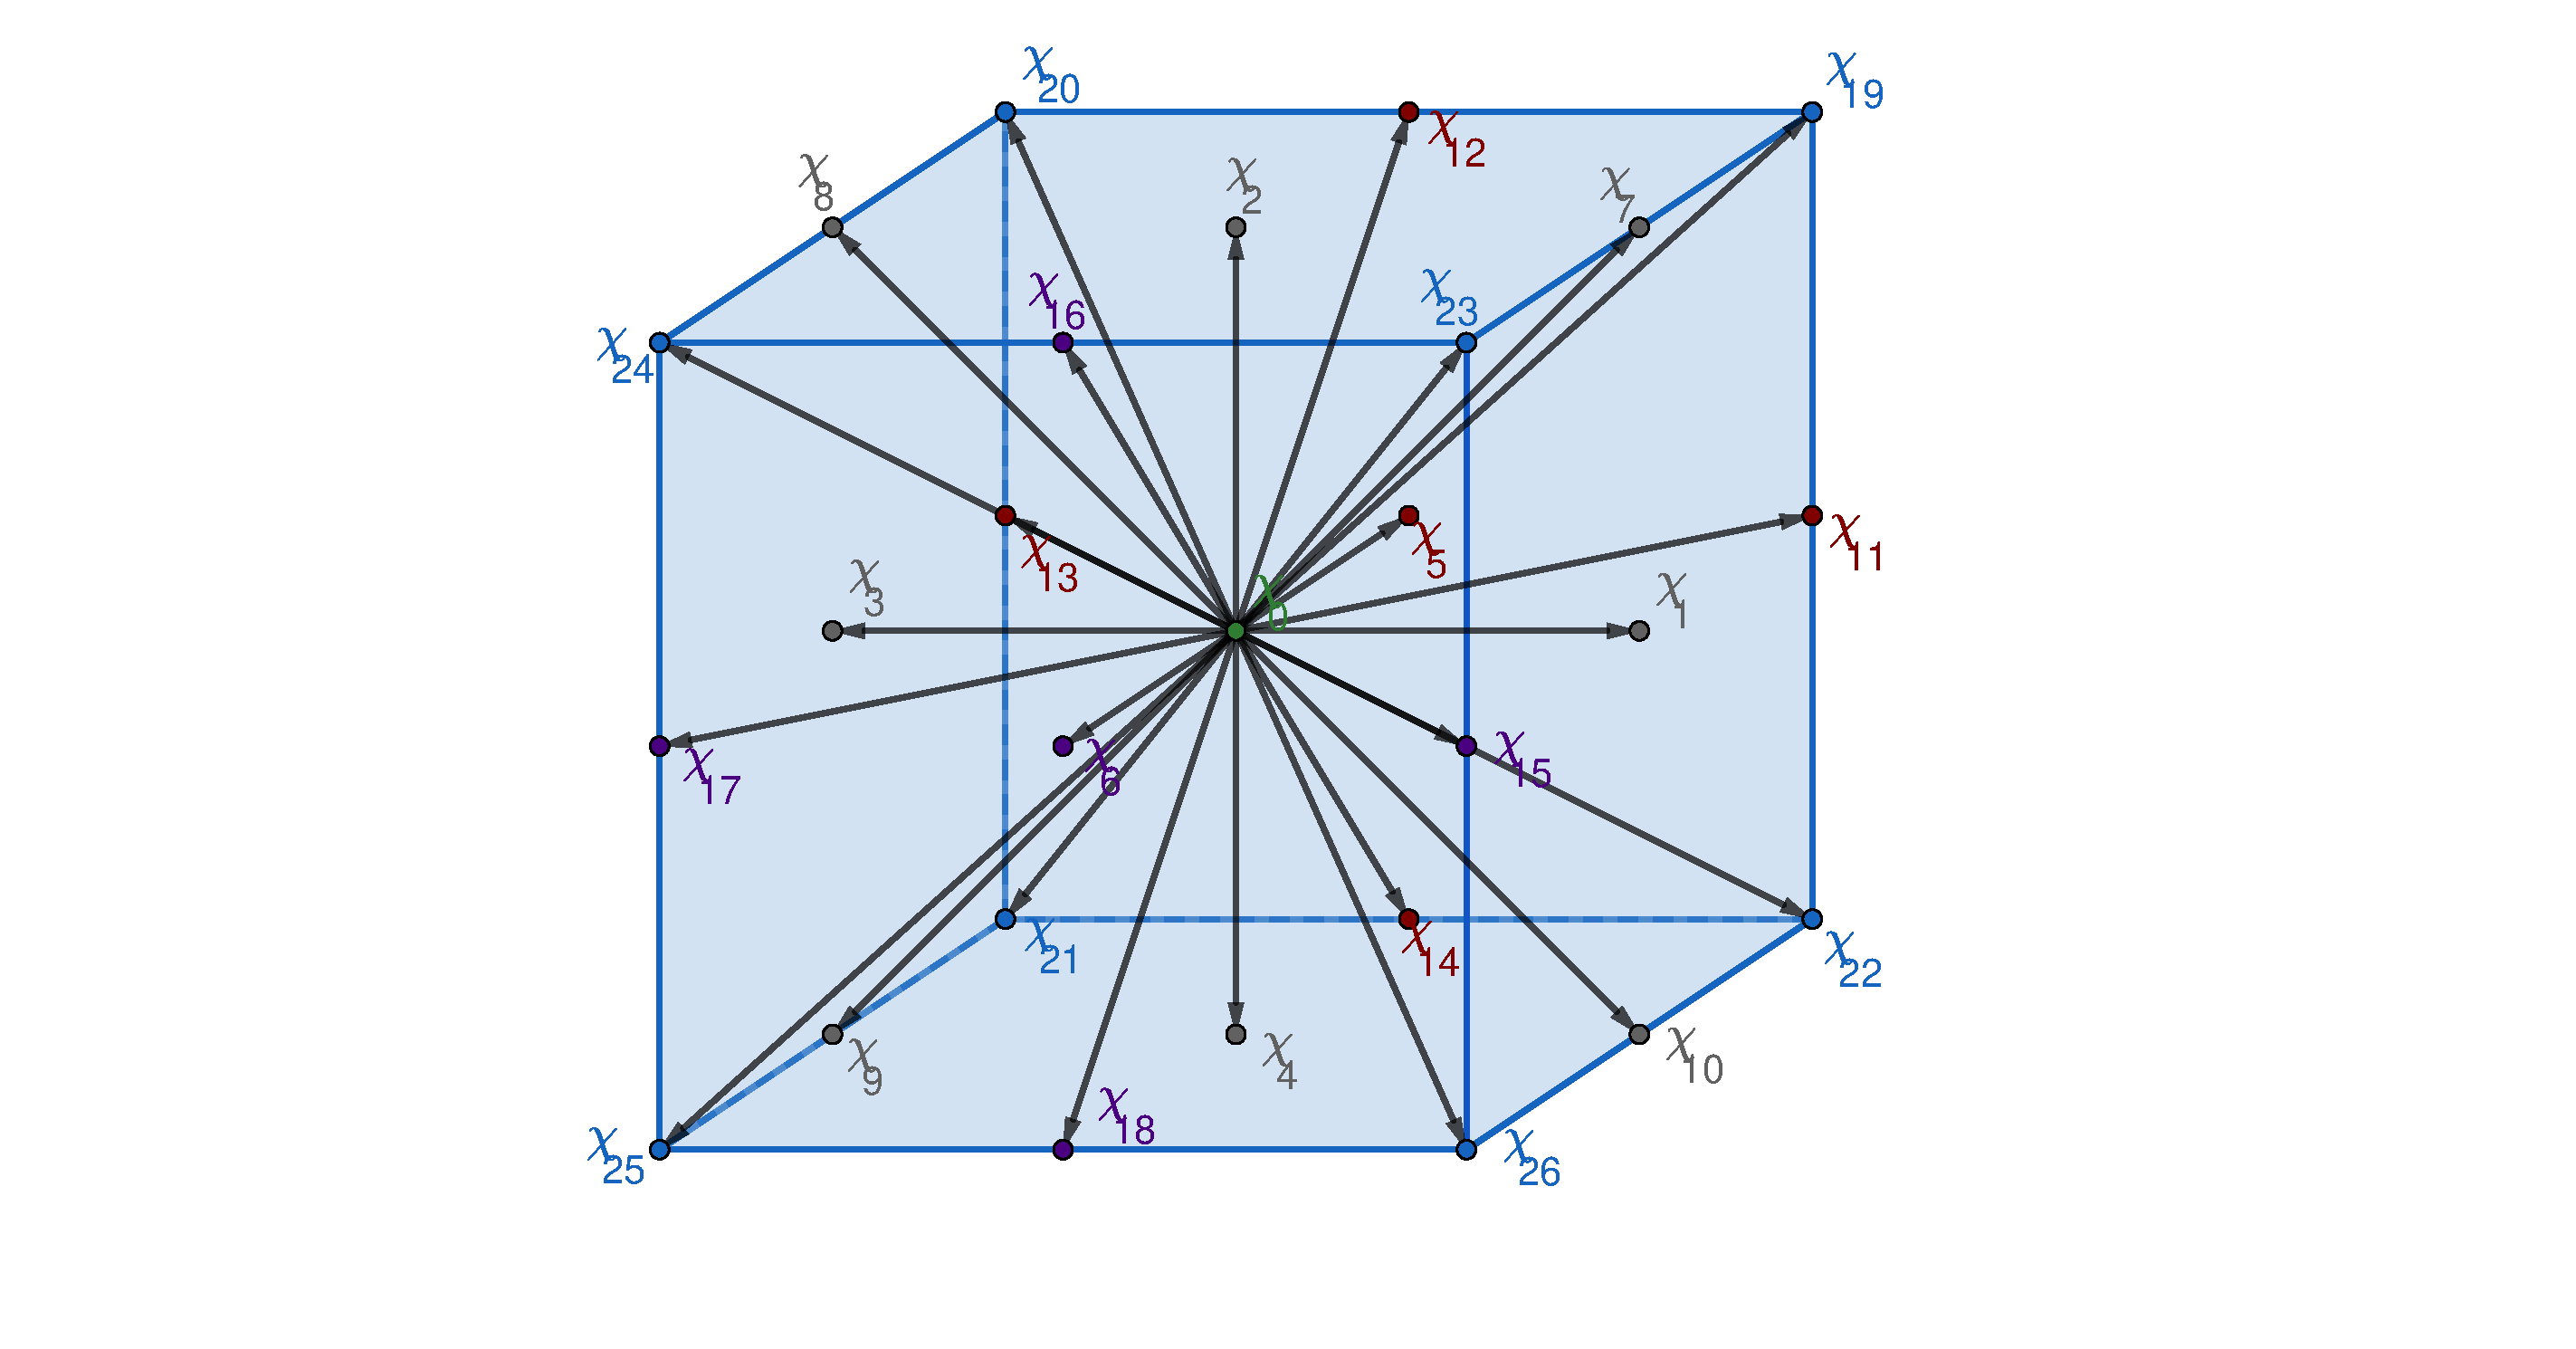
\includegraphics[scale = 0.3]{D3Q19.pdf}
\caption{Elección de los vectores y malla elegida para el sistema bidimensional en el flujo de Poiseuille }
\label{Poiseuille_100}
\end{figure}

la elección mostrada en la anterior figura define $w_{1}=w_{2}=w_{3}=w_{4}=w_{a}$ por otra parte $w_{5}=w_{6}=w_{7}=w_{8}=w_{b}$ obtenemos el siguiente sistema 

\begin{eqnarray}
\sum_{i}w_{i} &=& w_{o}+4w_{a}+4w_{b} = 1\\
\sum_{i}w_{i}\xi^{2}_{i\alpha}&=&\left(\frac{\Delta x}{\Delta t}\right)^{2}(2w_{a}+4w_{b})=c_{o}^{2}\\
\sum_{i}w_{i}\xi_{ix}^{2}\xi_{iy}^{2}&=&\left(\frac{\Delta x}{\Delta t}\right)^{4}4w_{b} = c_{o}^{4}\\
\sum_{i}w_{i}\xi_{i\alpha}^{4} &=& \left(\frac{\Delta x}{\Delta t}\right)^{4}(2w_{a}+4w_{b})=2c_{o}^{4}
\end{eqnarray}

En donde se obtiene

\begin{eqnarray}
c_{o}=\frac{\Delta x}{\Delta t} \frac{1}{\sqrt{3}}, \quad w_{o}=\frac{4}{9}, \quad w_{a} = \frac{1}{9},\quad w_{b}= \frac{1}{36}
\end{eqnarray}


\begin{figure}[H]
\label{perfiles}
\centering
\begin{subfigure}
\centering
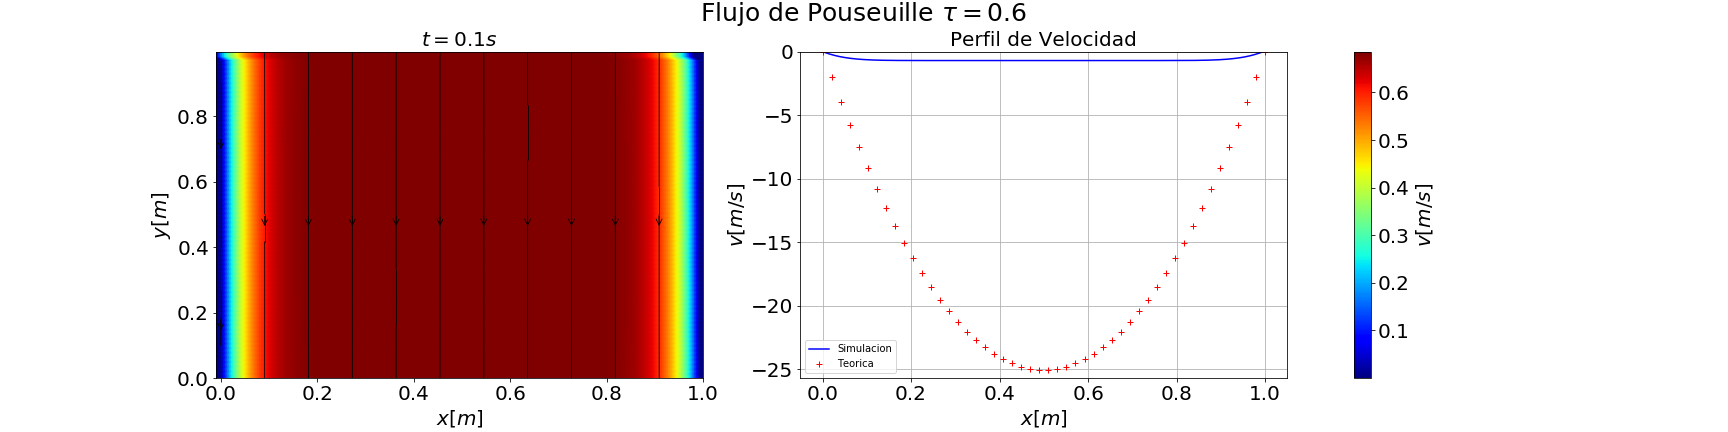
\includegraphics[scale=0.32]{01s.png} 
%\caption{Generic} \label{fig:timing1}
\end{subfigure}

\begin{subfigure}
\centering
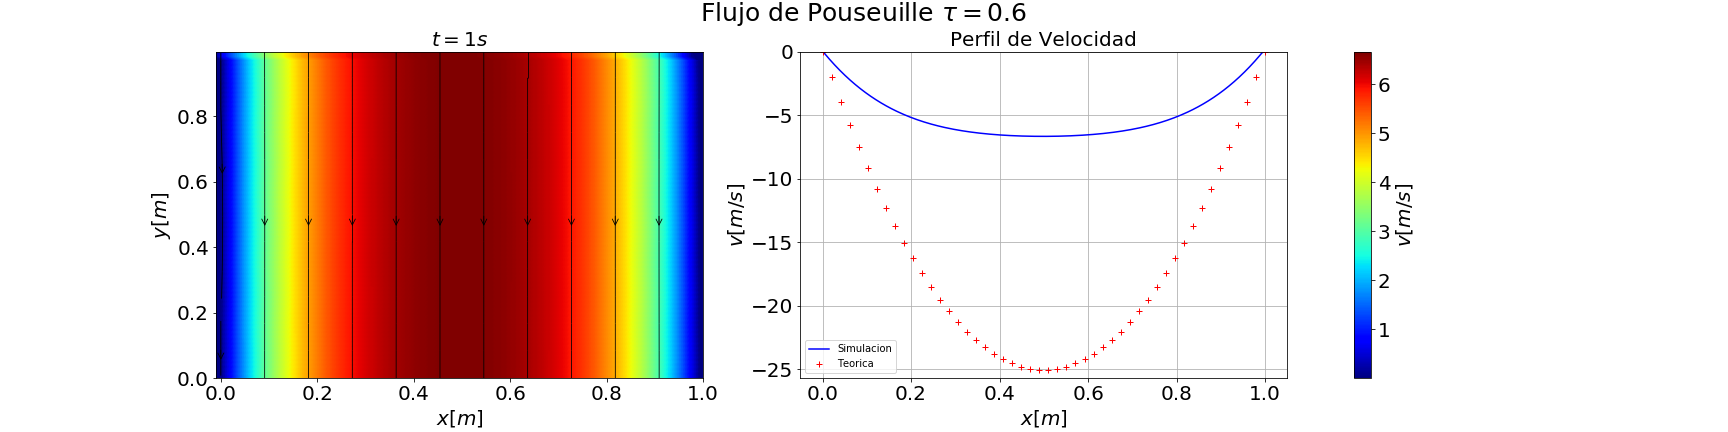
\includegraphics[scale=0.32]{1s.png} 
%\caption{Competitors} \label{fig:timing2}
\end{subfigure}

\begin{subfigure} 
\centering
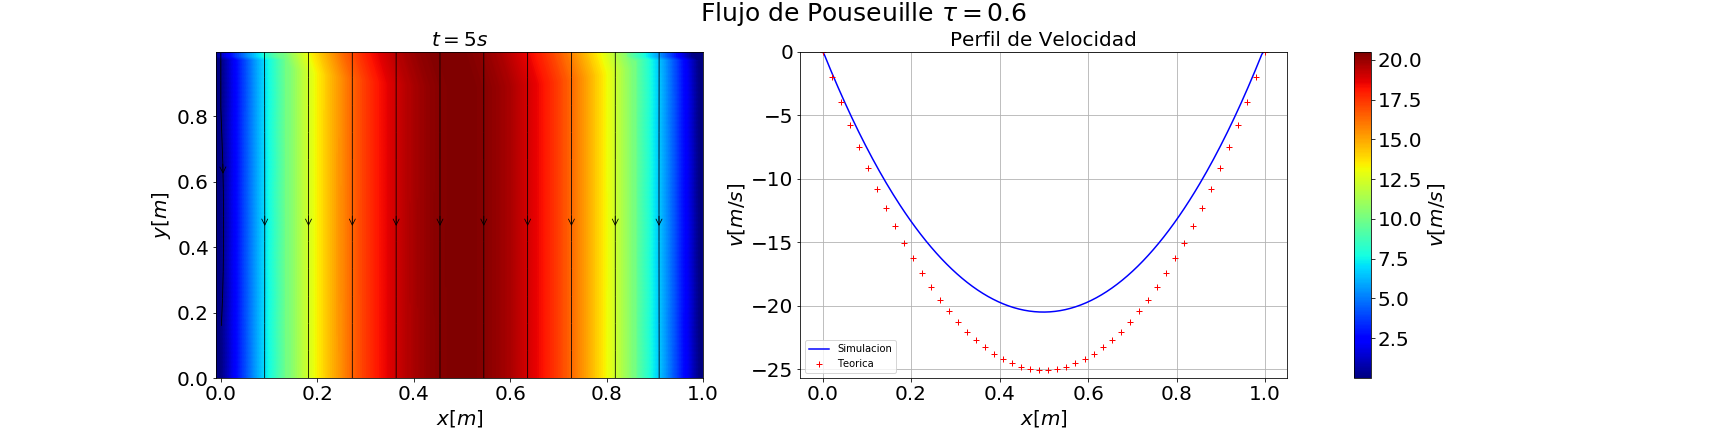
\includegraphics[scale=0.32]{5s.png} 
%\caption{Price regulation} \label{fig:timing3}
 \end{subfigure}
 
\begin{subfigure}
\centering
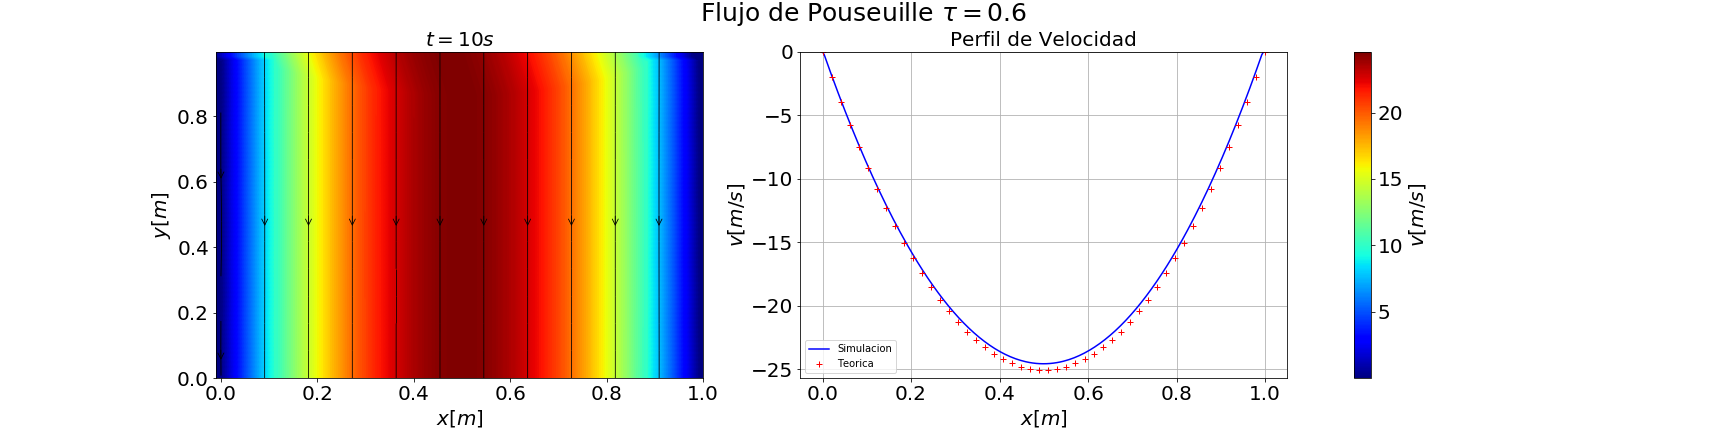
\includegraphics[scale=0.32]{10s.png} 
%\caption{Price regulation} \label{fig:timing3}
 \end{subfigure}

 \caption{Resultados simulación implementada en lattice Boltzmann para el flujo de Pouiseuille}


\end{figure}


\noindent para elegir las cantidades adecuadas al momento de representar las cantidades físicas reales , se ataca el problema de la siguiente manera. Denotando las unidades de lattice con el súper índice $^{*}$ . Dado que se conoce la solución teórica planteada en  \eqref{TeoricaPoiseuille} y teniendo en cuenta la ley de Poiseuille 

\begin{eqnarray}
u^{*} = \frac{g^{*}d^{*}}{8\nu^{*}}
\end{eqnarray}

\noindent se puede fijar $u^{*}=0.1$ para asegurar la stabilidad del código \cite{kruger}. Conocemos entonces el valor de la viscocidad en unidades de lattice y está dada de la siguiente manera

\begin{eqnarray}
\nu^{*} = (c_{o}^{*})^{2}\left(\tau^{*}-\frac{1}{2}\right)
\end{eqnarray}

\noindent entonces para encontrar el valor $\nu^{*}$ = 1/30, se elige $\tau =0.6$, esta elección determina las unidades correctas, para un sistema estable,  de la gravedad en unidades de lattice, obteniendose un valor del orden $g^{*} \approx 4\times 10^{-7}$. Además también se puede encontrar el número de Reynolds del sistema, encontrando

\begin{eqnarray}
Re = \frac{l^{*}u^{*}}{\nu^{*}} = \frac{lu}{\nu} =771
\end{eqnarray}

\noindent y desde acá se encuentra el paso de tiempo físico, dado por 

\begin{eqnarray}
\Delta t =(c_{o}^{*})^{2}\left(\tau^{*}-\frac{1}{2}\right)\frac{\Delta x^{2}}{\nu} =1.5\times 10^{-5}s
\end{eqnarray}

\noindent es decir que para que obtengamos el paso de tiempo de $t = 1s$, el sistema tiene que dar aproximadamente $66.000$ iteraciones. 

\medskip

\noindent para poder validar la simulación debemos comparar el resultado teórico y el resultado del perfil de velocidades obtenido en la simulación, esto se hace en la figura \ref{perfiles}, teniendo en cuenta que los factores de escala del sistema están dado por $dx = 1/256$ m, $1.5\times 10^{-5}$s. Esto asegura la validez del modelo planteado.


\subsection{Fluido en un cavidad}

Se presenta un flujo estacionario 2D en una cavidad cuadrada, utilizando el modelo lattice botlzmann con un lattice D2Q9. Este ejemplo es de mucha importancia dado que busca encontrar la validación del código a trevés de resultados conocidos. La configuración de este problema se muestra a continuación 


\begin{figure}[H]
\centering
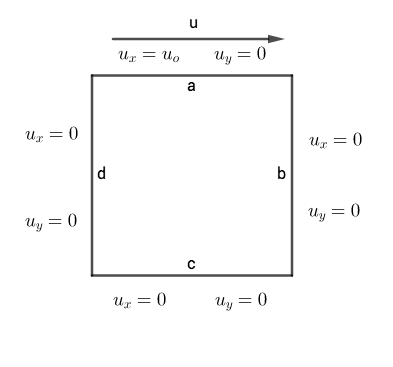
\includegraphics[scale = 0.6]{cavidad.png}
\caption{Esquema para el fluido en una cavidad}
\label{Poiseuille_100}
\end{figure}

\noindent El fluido está caracterizado por considerar un velocidad en el eje $x$ en la cara $a$, con magnitud $u_{o}$. El sistema está caracterizado por el número de Reynolds $Re = Lu_{o}/\nu$, donde $L$ es el lado del cuadrado ABCD y $\nu$ la viscosidad cinemática del fluido. Para las condiciones de frontera se utiliza el tradicional método bounce back \cite{kruger}. Para encontrar el número de Reynolds en la simulación se utiliza la expresión encontrada desde las ecuaciones de Navier Stokes partiendo del analisis de lattice Boltzmann

\begin{eqnarray}
Re = \frac{l u_{o}}{c_{o}^{2}(\tau - 0.5)}
\end{eqnarray}

\noindent En la simulación el tamaño del Lattice es de 256 x 256 y la velocidad de lado $a$ del cuadrado es $u_{o}= 0.1$, en donde el número de reynolds depende del tiempo de relajación. Los resultados obtenidos se presentan en las figuras siguientes

\begin{figure}[H]
\label{fig:Cavidad}
  \centering
  \begin{minipage}[b]{0.4\textwidth}
    \label{cavidadRe400}
    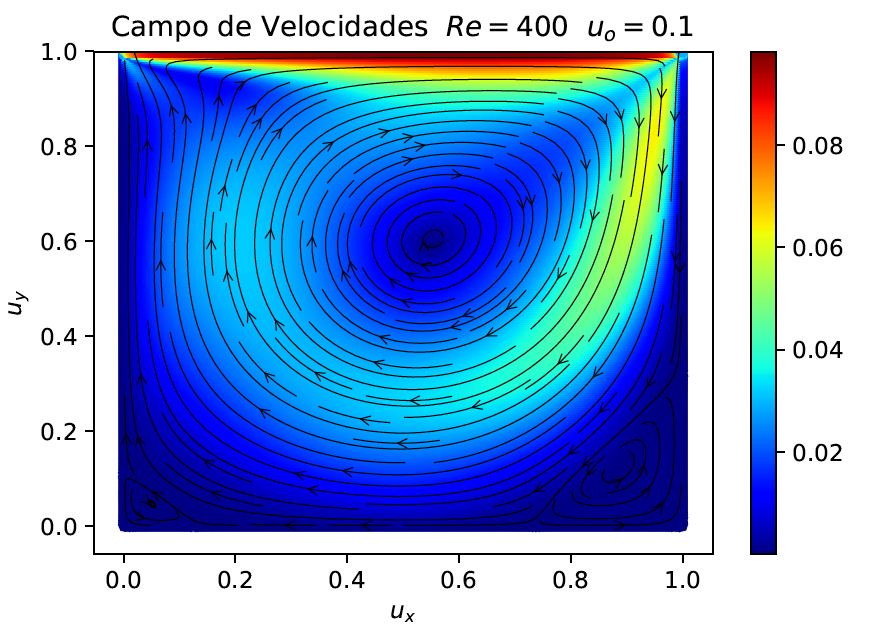
\includegraphics[scale =0.25]{cavidadRE400.png}
    %\caption{Fluido en una cavidad con un número de Reynolds de $Re = 400$}
  \end{minipage}
  \hspace{1cm}
  \begin{minipage}[b]{0.4\textwidth}
  \label{cavidadRe2000}
    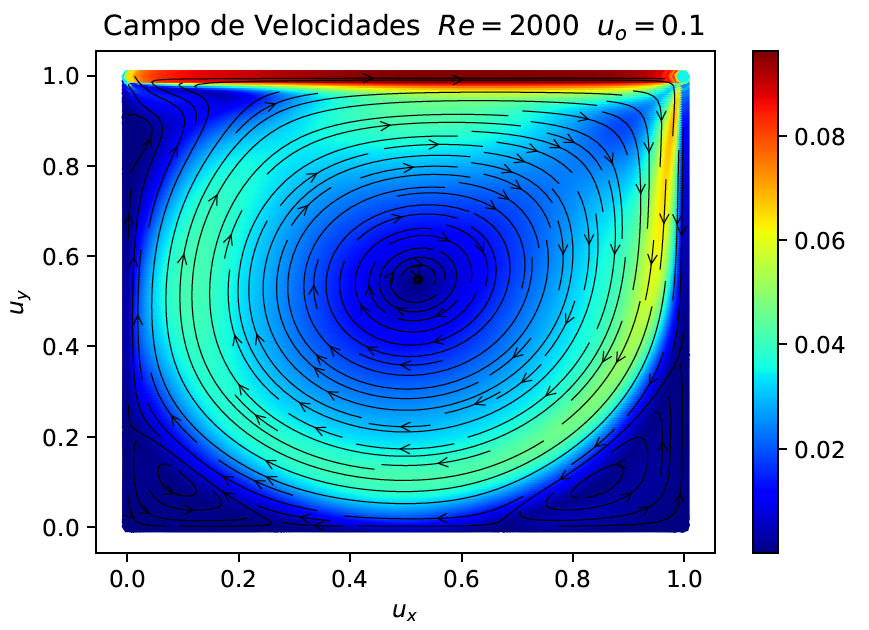
\includegraphics[scale=0.25]{cavidadRE200.png}
    %\caption{Fluido en una cavidad con un número de Reynolds de $Re = 2000$}
  \end{minipage}
  \caption{Fluido en una cavidad cuadrada con velocidad $u_{x} = 0.1$}
\end{figure}

Las lineas de corriente que se obtuvieron muestran claramente la formación de tres vórtices, uno principal en el centro del cuadrado y dos en las esquinas contrarias, es decir en el lado $c$. El efecto del número de Reynolds es claro al comparar los resultados en cuanto más grande sea tal número la tendencia a formar vórtices dentro del fluido es más grande\footnote{El código implementado se puede encontrar en el siguiente \href{https://github.com/jomen93/Cavidad_2D}{link}}.



\newpage









